\begin{latin}
\textbf{Solution}: In merge sort, the $n$ element array is divided into two halves each with $\frac{n}{2}$ elements (for $n$ = even), or one with $\dfrac{n}{2}$ and the other with $\frac{n}{2}+1$ elements. The two halves are sorted and merged. The algorithm for performing merge sort is as follows:
\begin{figure}[h!]
\centerline{ 
\includegraphics[width=12cm,height=18cm]{2.jpg}}
%\caption{ }
%\label{1.jpg}      
\end{figure}\\

The algorithm Merge$(\min, m, \max)$ is performed in $O(n)$. The algorithm mergeSort $(int
\min, int \max)$ of $n$ element becomes half when it is called recursively. Thus, the whole algorithm
takes
\begin{align*}
T(n) &\leq 2 T (\frac{n}{2})+cn \\
&\leq 2 \bigg[ 2 T (\frac{n}{2^2}) + c \frac{n}{2} \bigg] + cn\\
T(n) &\leq 2^2 T (\frac{n}{2^2})+2cn \\
\cdots \\
\cdots 
\end{align*}
\begin{align*}
&T(n)\leq 2^i T (\frac{n}{2^i})+icn \\
& if ~~2^i=n, i=\log_2 n \\
&T(n) \leq  2^i T(1) + cn \log_2 n
\end{align}
$T(1) = 1$ (time required to sort a list of one element).\\
Thus, the complexity of merge sort is $O(n \log_2 n)$.\\
$3.$ Prove that the k clique problem is $NP$ complete.\\
\textbf{Solution:}
\begin{Definition}
Given a graph $G = {V, E}$ and an integer $k$, check whether there exists a sub-graph $C$
of $G$ which contains $k$ number of vertices.
\end{Definition}
(The max clique problem is fi nding a clique with largest number of vertices. It is an $NP$ hard
problem.)\\
To prove that clique is $NP$ complete, we need to prove:\\
\textbf{A. Clique is NP}\\
$\square$ Check whether $C$ contains $k$ number of vertices. This can be done in $O(| C |)$.\\
$\square$ Check whether $C$ is a complete sub-graph. This can be done in $kC_2$ steps.\\
Thus, checking whether $C$ is a clique of $G$ or not can be performed in polynomial time.
A graph with $n$ number of vertices can have $2n$ number of such vertex combination. For each
of the combinations, the same checking algorithm is performed. Among these, the clique with $k$
vertices is the $ k$-clique of $G$. So, a $k$-clique algorithm is carried out by a non-deterministic Turing
machine in polynomial time. Hence, it is in $NP$.\\
\textbf{B. Reduce $3-SAT$ to $k$-clique}\\
\textbf{Reduction:}\\
$\square$ For each clause of a Boolean assignment, create distinct vertices for each literal. If a
Boolean assignment contains $C$ clauses, then the number of vertices is $3C$. \\
$\square$ Join the vertices of the clauses in such a way that\\
 – Two vertices of the same clause cannot be joined.\\
– Two vertices whose literals are the negation of the other cannot be joined.
\begin{exa}
Consider $F=(X_1 \vee X_2 \vee Y_1) \wedge (X_3 \vee \neg Y_1 \vee \neg Y_2) \wedge (X_4 \vee X_5 \vee \neg Y_2) $ \\
The graph is \\
\begin{figure}[h!]
\centerline{ 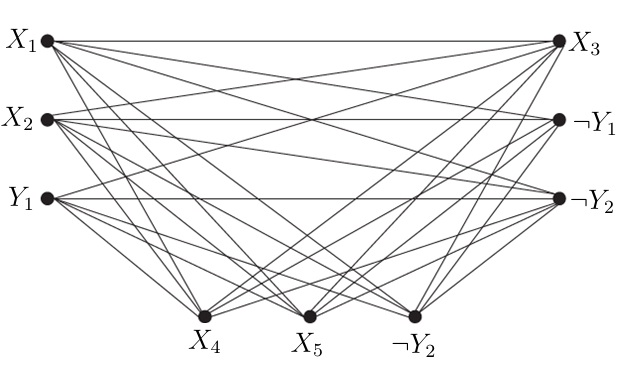
\includegraphics[width=13cm,height=7cm]{1.jpg}}
%\caption{ }
%\label{1.jpg}      
\end{figure}\\
If it can be proved that $G$ has a $k$-clique if and only if $F$ is satisfi able, then the reduction is correct.
\end{exa}
$\square$ \textbf{If F is satisfi able, G has k-clique: }If the $3-SAT$ instance $F$ is TRUE, then each clause is TRUE, which means every clause has a TRUE literal. By selecting a corresponding vertex to a TRUE literal in each clause, a clique in $G$ of size $k$ is constructed, where $k $ is the number of clauses of the $3-SAT$ instance. Because, if there is a missing edge, that would mean that our truth assignment effectively set something to be true and false at the same time ($Y_1$ and $\neg Y_1$)$!$
\\
$\square$ \textbf{If G-has k-clique, F is satisfi able:} Assume that there is a clique of size $k$ in $G$ where k is the number of clauses in $F$. It is to be proved that there must be a truth assignment that satisfies the given Boolean formula. Clique is a complete graph. Let us assume that the truth assignment induced by the labels of the vertices satisfies $F.$ It signifies that every pair of vertices in the clique has an edge. But the vertices labelling the literals may be set to both true and false. Already it is mentioned that every trio of vertices corresponding to a clause of $F$ have no edges between those vertices, which signifies that there must be a vertex from every clause of $F$ in the clique. This shows that the clauses of $F$ are satisfied as well as $F$  is satisfied.\\
This reduction is possible in polynomial time. Hence, clique is $NP$ complete.
\section*{Multiple Choice Questions}
$1.$ Worst case time complexity is denoted by
the notation. \\
a) Big oh notation\\
b) Big omega notation\\
c) Theta notation\\
d) Little omega notation\\
$2.$ Best case time complexity is denoted by the
notation.\\
a) Big oh notation\\
b) Big omega notation\\
c) Theta notation\\
d) Little omega notation\\
$3.$ if $f(n)=O(g(n))$ and $f(n)=\Omega(g(n))$, then which is true?\\
a) $f(n)=\omega (g(n))$~~~~~b) $f(n)=o(g(n))$ \\
c) $f(n)=\Theta(g(n))$~~~~~~d) $f(n)=\theta(g(n))$\\
$4.$ The problem which results in ‘yes’ or ‘no’ is \\
a) Decision problem\\
b) Optimization problem\\
c) Search problem\\
d) Functional problem\\
$5.$ Which type of problem is the shortest path
algorithm?\\
a) Decision problem\\
b) Optimization problem\\
c) Search problem\\
d) Functional problem\\
$6.$ Which is true for the $P$ class problem?\\
a) The number of steps (or time) required
to complete the algorithm is a polynomial
function of $n$.\\
b) It is computable by a deterministic
Turing machine in polynomial time.\\
c) It contains all sets in which the membership
may be decided by an algorithm
whose running time is bounded by a
polynomial.\\
d) All of these\\
\textbf{Answers:} $1.$a   \quad   $2.$b   \quad   3.c  \quad  4.a   \quad  5.b      \quad 6.d
\section*{GATE Questions}
1. For problems $X$ and $Y$, $ Y$ is $NP$ complete and $X$  reduces to $Y$ in polynomial time. Which of the following is true? \\
a) If $X$ can be solved in polynomial time, then so can $ Y$.\\
b) $X$ is $NP$ complete\\
c) $X $ is $NP$ hard\\
d) $ X $ is in $NP$, but not necessarily $NP$ complete.\\
2. Which of the problems is not $NP$ hard?\\
a) Hamiltonian circuit problem \quad \quad \quad \quad \quad \quad \quad \quad b) The $0/1$ knapsack problem \\
c) Finding bi-connected components of a graph \quad  d) The graph colouring problem \\
3. Ram and Shyam have been asked to show a certain problem $\Pi$  is $NP$ complete. Ram shows
a polynomial time reduction from $3-SAT$ problem to $\Pi$, and Shyam shows a polynomial time
reduction from $\Pi$ to $3$ SAT. Which of the following can be inferred from these reductions?\\
a) $\Pi$ is $NP$ hard but not $NP$ complete     \quad \quad b)$\Pi$ is $NP$, but is not $NP$ complete\\
c) $\Pi$ is $NP$ complete    \quad \quad \quad \quad \quad \quad \quad \quad \quad  d) $\Pi$ is neither $NP$ hard nor $NP$\\
4. No body knows yet if $P = NP$. Consider the language $L $defined as follows.
\begin{center}
$L=\begin{cases}
(0+1)^* \quad  \quad   if ~~P=NP \\
\varphi \quad \quad \quad \quad \quad Otherwise
\end{cases}$
\end{center}
Which of the following statements is true?\\
a) $L$ is recursive\\
b) $L$ is recursively enumerable but not recursive \\
c) $L$ is not recursively enumerable \\
d) Whether $L$ is recursive or not will be known after we find out if $P = NP$

\end{latin}
